\chapter{Функціональні завдання, які вирішує система}
\label{ch:functional_tasks}

Даний розділ присвячено опису ключових функціональних завдань, які користувачі можуть вирішувати за допомогою веб-платформи для комунікації та обміну знаннями в спільноті бджолярів \textit{Beekeepers Community Platform}. Опис кожного завдання супроводжується ілюстраціями інтерфейсу, що демонструють відповідні можливості системи.

\section{Забезпечення доступу та управління обліковим записом}
\label{sec:tasks_auth}
Платформа надає механізми для реєстрації нових користувачів та безпечної автентифікації існуючих, а також базові можливості для управління власним профілем.

\subsection{Реєстрація нового користувача в системі}
\label{subsec:task_registration}
Система дозволяє потенційним учасникам спільноти створювати нові облікові записи. Процес реєстрації включає наступні етапи:
\begin{enumerate}
    \item Користувач переходить на сторінку реєстрації, де йому пропонується заповнити форму.
    \item Необхідно вказати актуальну електронну адресу, обрати унікальне ім\'я користувача (username) та створити пароль. На рисунку \ref{fig:task_registration_form} показано вигляд даної форми.
    \item Після надсилання форми, система виконує валідацію введених даних. У разі успіху створюється новий обліковий запис, а на вказану електронну пошту надсилається лист із посиланням для верифікації.
    \item Активація облікового запису відбувається шляхом переходу за верифікаційним посиланням, що підтверджує володіння вказаною електронною адресою.
\end{enumerate}

\begin{figure}[htbp]
    \centering
    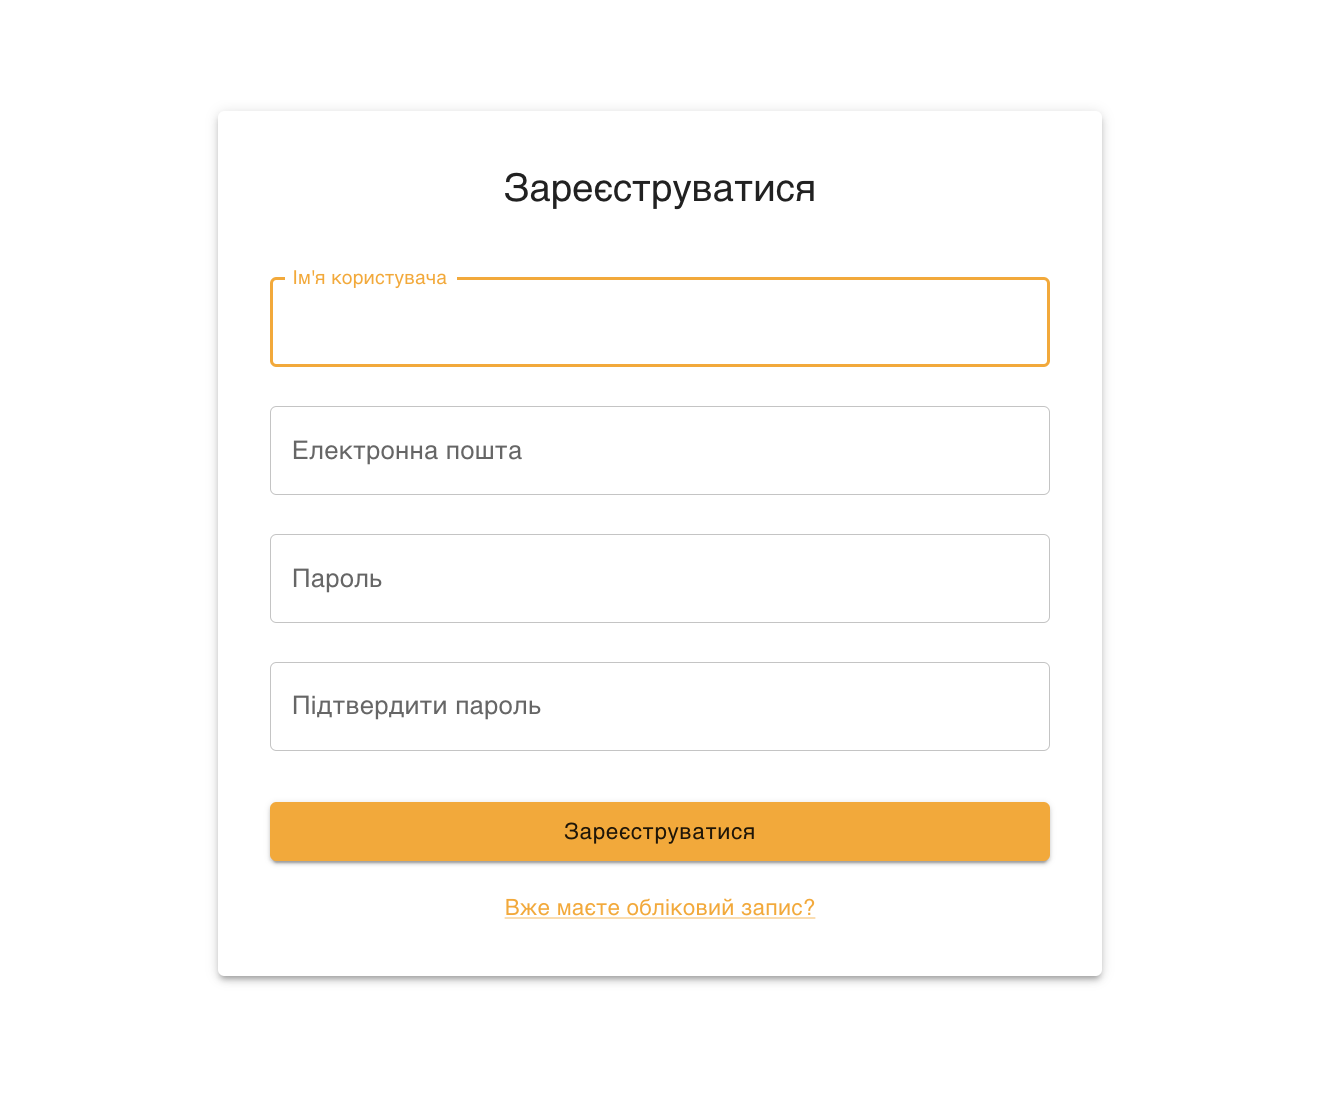
\includegraphics[width=0.6\textwidth]{practice_report/images/registration_form.png}
    \caption{Інтерфейс форми для реєстрації нового користувача}
    \label{fig:task_registration_form}
\end{figure}

% TODO: (from old appendix) Add text and screenshot for email verification page/prompt interface here if desired

\subsection{Автентифікація користувача в системі}
\label{subsec:task_login}
Для доступу до функціоналу платформи зареєстровані користувачі повинні пройти процедуру автентифікації:
\begin{enumerate}
    \item Користувач відкриває сторінку входу до системи (див. рисунок \ref{fig:task_login_page}).
    \item Система надає можливість ввести електронну пошту та пароль, вказані при реєстрації.
    \item Після натискання кнопки "Увійти", система перевіряє облікові дані. У разі успіху користувач отримує доступ до платформи.
    \item Також реалізована можливість швидкої автентифікації за допомогою існуючого облікового запису Google, що спрощує процес входу.
\end{enumerate}

\begin{figure}[htbp]
    \centering
    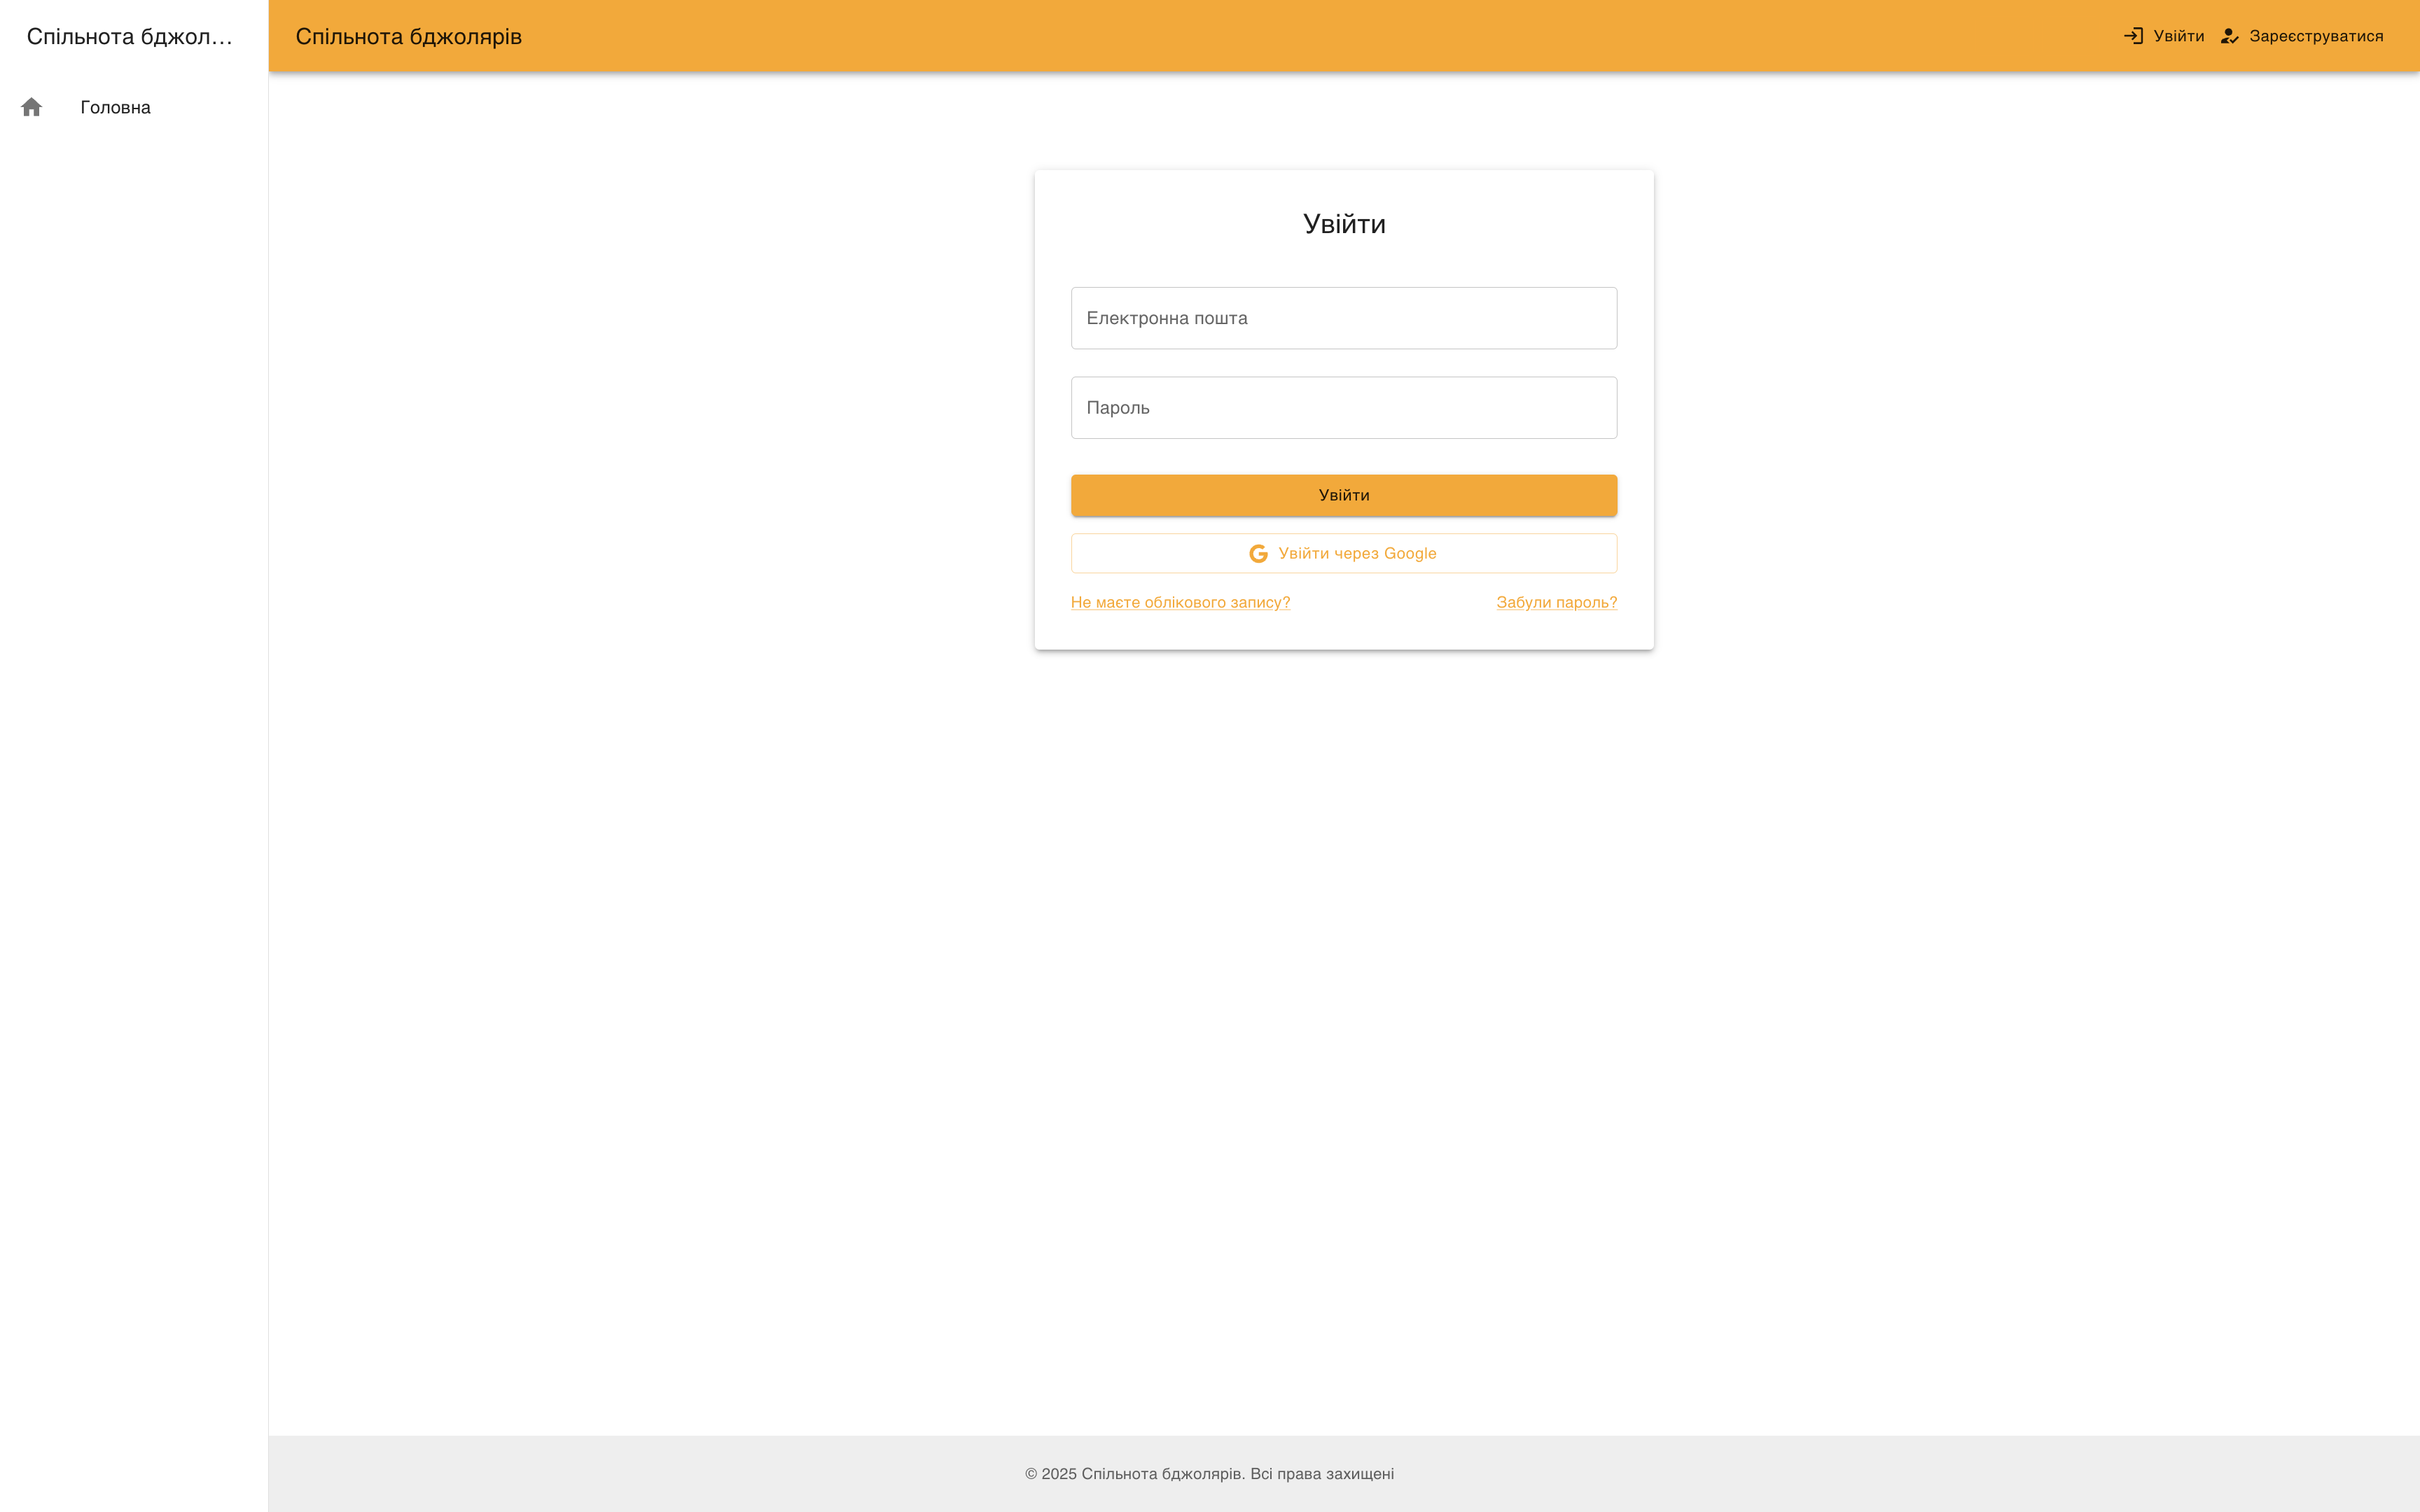
\includegraphics[width=0.6\textwidth]{practice_report/images/login_page.png}
    \caption{Інтерфейс сторінки для входу до системи}
    \label{fig:task_login_page}
\end{figure}

% TODO: (from old appendix) Add text and screenshot for what happens after successful login (e.g., dashboard or main page view)

\section{Управління геопросторовими даними пасік та полів}
\label{sec:tasks_map}
Одним з ключових завдань, яке вирішує платформа, є надання інструментів для візуалізації та управління геопросторовою інформацією, важливою для бджолярів.

\subsection{Візуалізація та менеджмент вуликів}
\label{subsec:task_map_hives}
Система дозволяє користувачам управляти інформацією про власні вулики на інтерактивній карті:
\begin{itemize}
    \item \textbf{Додавання вулика:} Користувач може розмістити маркер вулика на карті, вказавши його місцезнаходження, та заповнити атрибутивну інформацію (назва, нотатки) через діалогове вікно.
    \item \textbf{Відображення вуликів:} Вулики відображаються на карті за допомогою спеціальних іконок. При виборі маркера вулика користувач бачить детальну інформацію у спливаючому вікні, як показано на рисунку \ref{fig:task_map_hives_demo}.
    \item \textbf{Видалення вулика:} Система надає можливість видалити інформацію про вулик з карти та бази даних (з підтвердженням операції).
\end{itemize}

\begin{figure}[htbp]
    \centering
    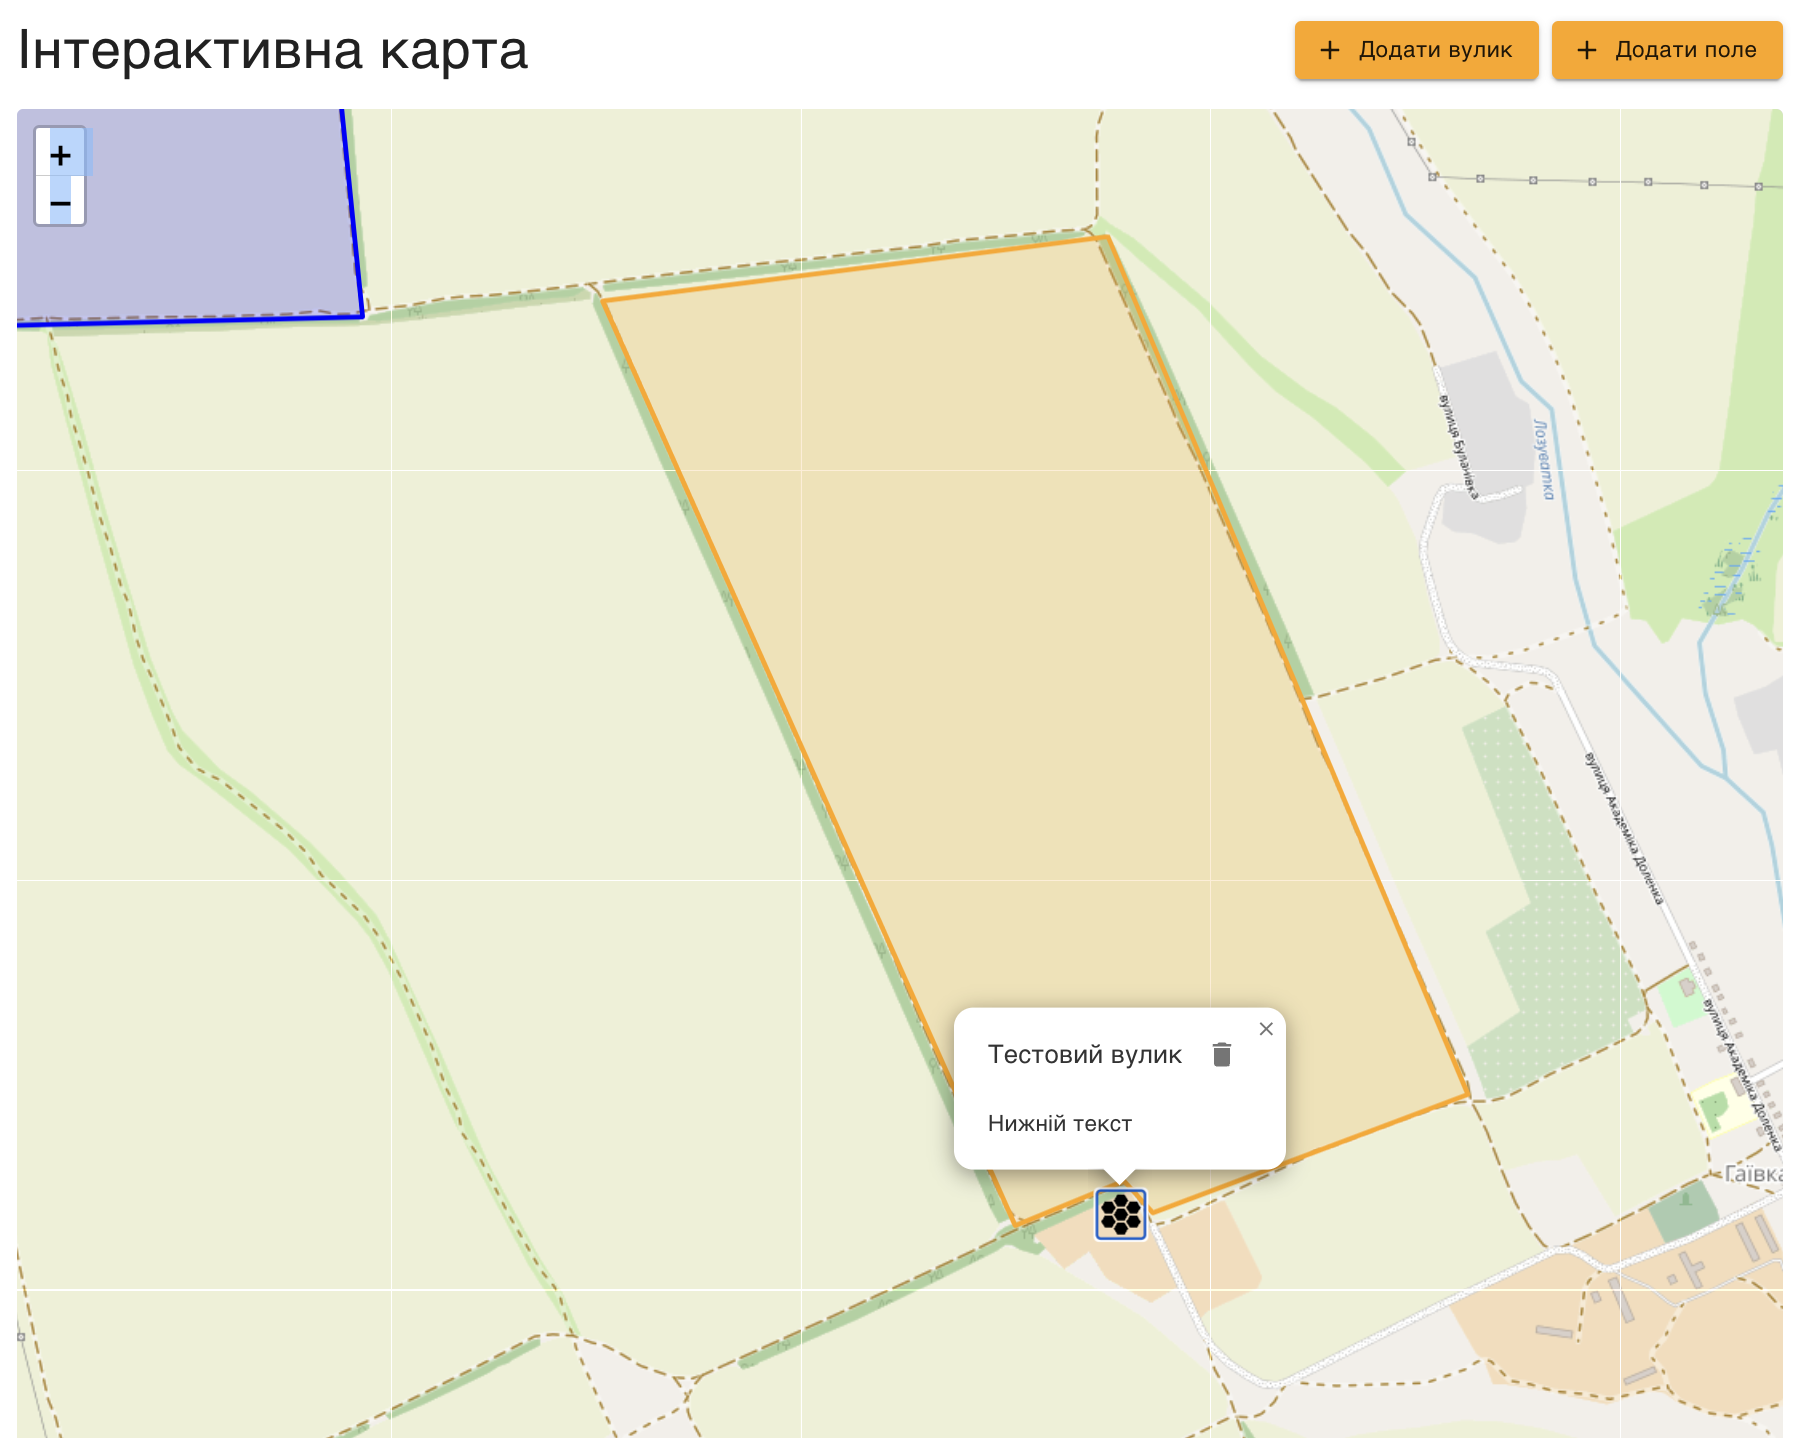
\includegraphics[width=0.8\textwidth]{practice_report/images/map_hives_demo.png}
    \caption{Відображення маркерів вуликів та інформаційного вікна на карті}
    \label{fig:task_map_hives_demo}
\end{figure}

% TODO: Add sections for Adding Hives (screenshot of dialog), Deleting Hives (screenshot of confirmation) from user manual perspective

\subsection{Візуалізація та менеджмент сільськогосподарських полів}
\label{subsec:task_map_fields}
Платформа надає функціонал для роботи з даними про сільськогосподарські поля:
\begin{itemize}
    \item \textbf{Додавання поля:} Користувач може окреслити межі поля на карті (полігон) та ввести його характеристики (назва, тип культури, період цвітіння, заплановані дати обробки) через відповідне діалогове вікно.
    \item \textbf{Відображення полів:} Поля візуалізуються на карті полігонами. При виборі поля відображається його атрибутивна інформація, включаючи дати обробок (див. рисунок \ref{fig:task_map_fields_demo}).
    \item \textbf{Індикація статусу обробки полів:} Система автоматично змінює колір полігону поля для візуального сповіщення про близькість запланованих хімічних обробок, що допомагає бджолярам оцінити ризики.
    \item \textbf{Редагування даних поля:} Надається можливість оновлювати метадані полів через спеціалізований інтерфейс.
\end{itemize}

\begin{figure}[htbp]
    \centering
    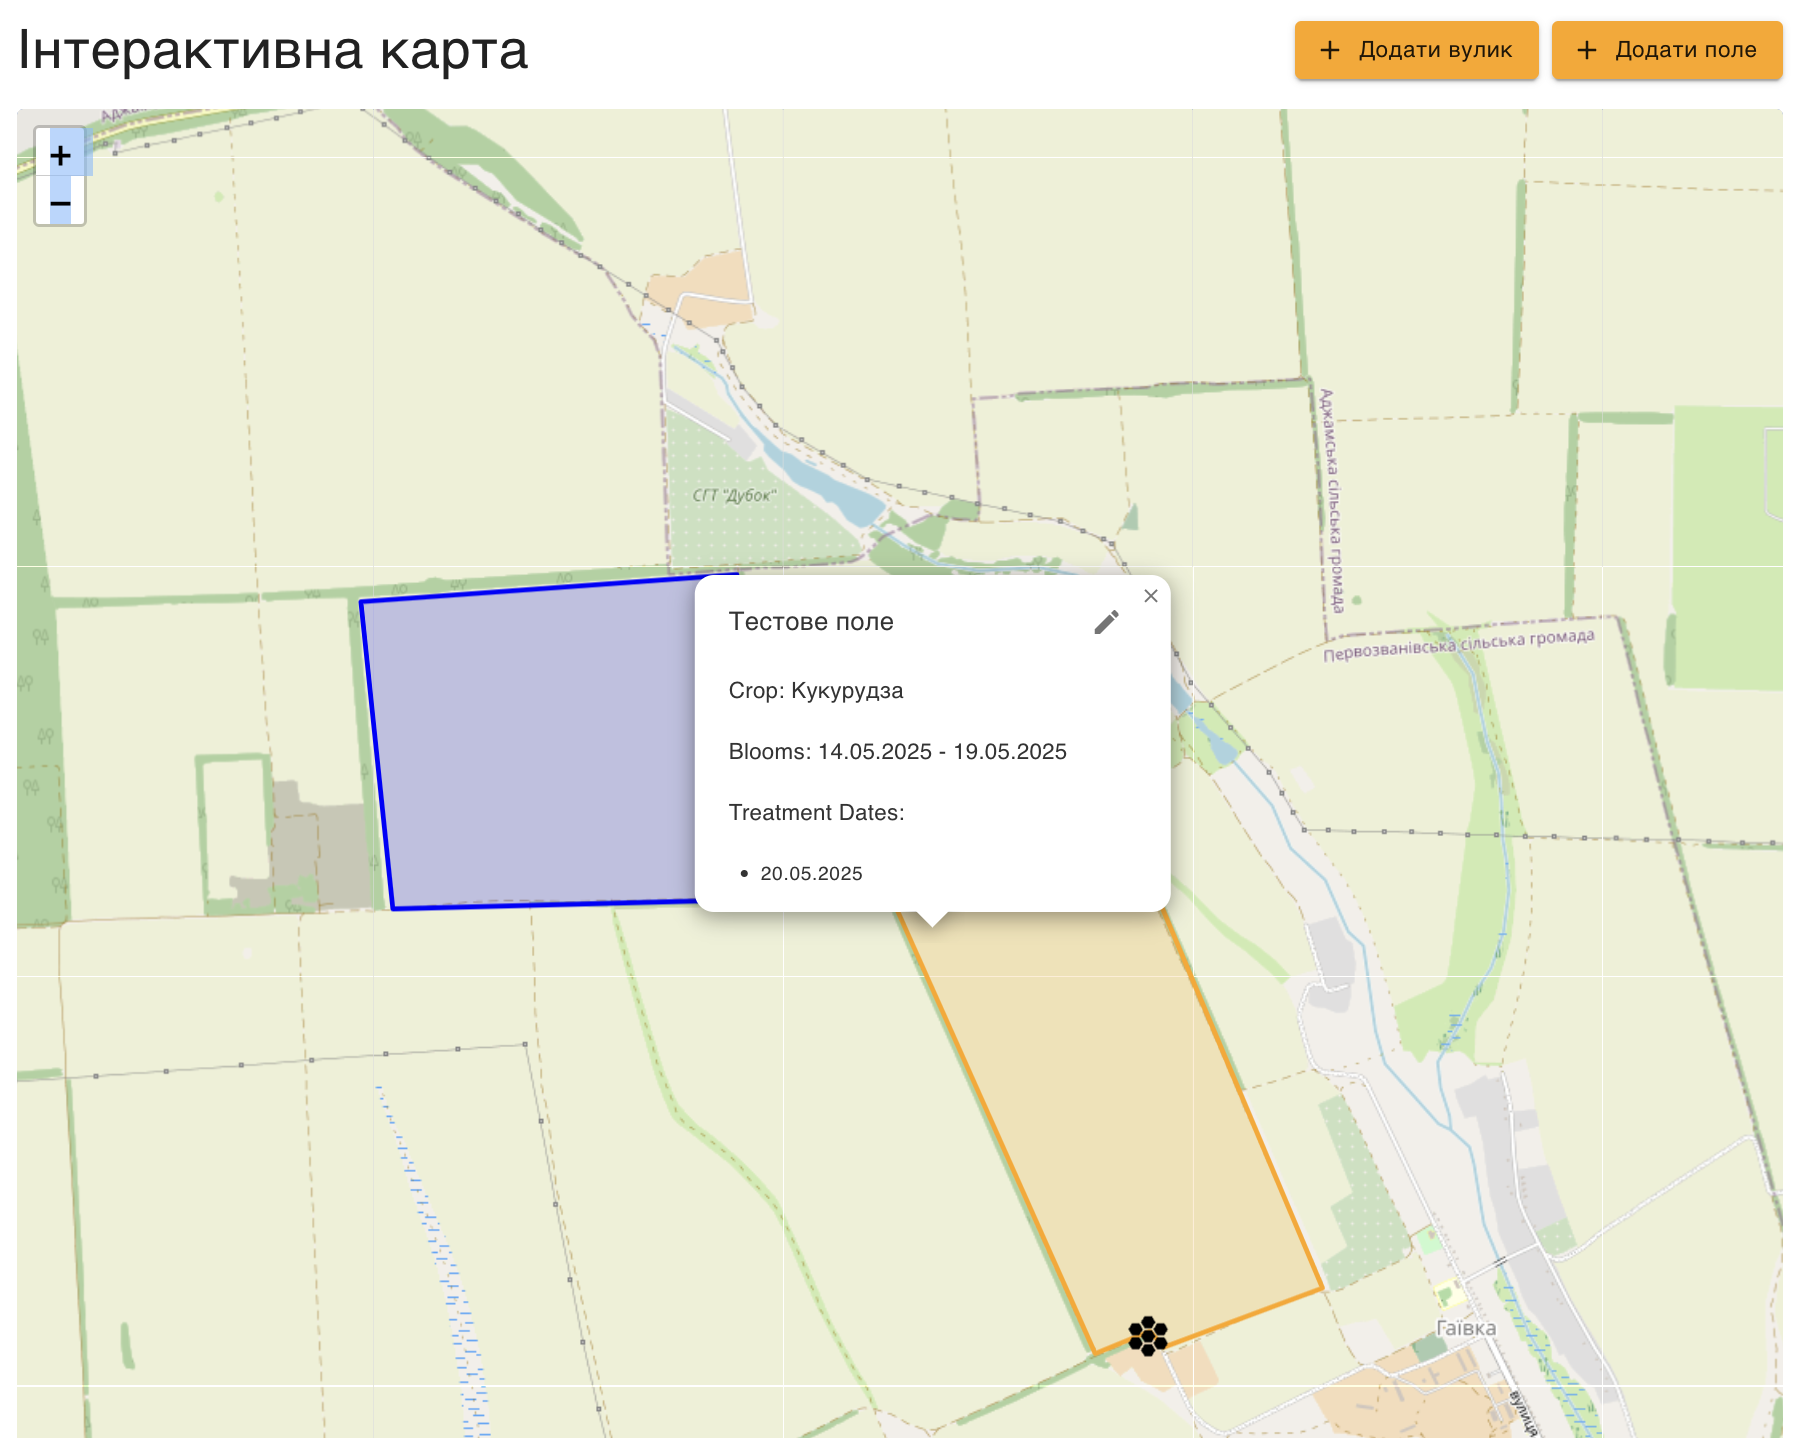
\includegraphics[width=0.8\textwidth]{practice_report/images/map_fields_demo.png}
    \caption{Відображення полігонів полів та інформаційного вікна на карті}
    \label{fig:task_map_fields_demo}
\end{figure}

% TODO: Add sections for Adding Fields (dialog), Editing Fields (dialog), Deleting Fields (confirmation) from user manual perspective

% TODO: Add sections for Forum, Knowledge Base/FAQ, User Profile Management here, adapted from appendix_user_manual.tex 